\chapter{Results: Comparing CDA and FBA}
\label{ch:results}

\begin{quote}
\small
\textbf{Scope of this chapter.} Every number and figure below comes from
one executed run: the SOL perpetual, the full month of 1--31~December 2025,
$\tau = 1$\,second, and the single fixed engine configuration of
\Cref{app:config}. Throughout, a \textbf{bucket} is one of the 2,678,400
consecutive one-second windows of the month, and every metric is computed
per bucket. Each paired difference (FBA$-$CDA) uses only the buckets in
which the metric exists for \emph{both} engines (the $n$ column) and a
Newey--West standard error (\Cref{sec:experiments}). Sections
\ref{sec:res21}--\ref{sec:res23} report the results, \Cref{sec:res_summary}
summarises them, and \Cref{sec:metricreliability} collects in one place
every limit on how far they can be read.
\end{quote}

\section{Sample and Descriptive Statistics}
\label{sec:sample}

\Cref{tab:sample} describes the replayed sample, the event stream that both
engines receive unchanged, so any difference in the results cannot come from
the input.

\begin{table}[htbp]
\centering
\caption[Sample description]{Description of the replayed sample. Message
counts refer to the raw event stream, identical for both engines; trade
counts and notional are each engine's own simulated output.}
\label{tab:sample}
\small
\begin{tabularx}{\textwidth}{@{}L c@{}}
\toprule
\textbf{Characteristic} & \textbf{Value}\\
\midrule
Instrument & SOL perpetual futures (SOL-PERP), Hyperliquid\\
Session & 1--31 Dec 2025 (\FbaEmptyBatchShare\% of 1s FBA batches empty)\\
Input files & \SampleFilesTotal\\
Total records seen & \SampleTotalMessages\\
\quad of which new live orders & \SampleNewOrders\\
\quad of which cancellations & \SampleCancellations\\
\quad of which other (rejections, fills, non-triggered conditionals) & \SampleOtherEvents\\
\quad skipped (zero size after rounding) & \SampleSkipped\ (\SampleSkippedPct\%)\\
Distinct participants (user ids) & \SampleDistinctParticipants\\
Median inter-arrival time, raw record stream & \SampleMedianInterArrival\,ms\\
Mean inter-arrival time & \SampleMeanInterArrival\,ms\\
99th pct.\ inter-arrival time & \SamplePNinetyNineInterArrival\,ms\\
CDA trades (simulated) & \SampleCdaTrades\\
FBA trades (simulated) & \SampleFbaTrades\\
CDA executed notional (simulated) & \$\SampleCdaNotional\\
FBA executed notional (simulated) & \$\SampleFbaNotional\\
\bottomrule
\end{tabularx}
\end{table}

The data have no separate modify event and neither engine implements one, so
a change to a resting order appears as some combination of the categories
above.

\textbf{Inter-arrival time} is the time between one record and the next. Its
median (\SampleMedianInterArrival\,ms) is exactly zero because
\SampleZeroGapPct\% of consecutive records have the same nanosecond timestamp,
as expected on a venue that processes orders block by block
(\Cref{sec:venue}). The mean (\SampleMeanInterArrival\,ms) and the 99th
percentile (\SamplePNinetyNineInterArrival\,ms) show the gaps between these
bursts, of tens to hundreds of milliseconds. This also explains the
empty-batch share: ``\FbaEmptyBatchShare\% of batches empty'' means that in
that second no buy limit reached any sell limit (a batch of only market
orders does not trade either, \Cref{sec:environment}), not that the second
was quiet.

\section{Validation Results}
\label{sec:validationresults}

These are preconditions, not findings: the comparison can only be trusted as
far as the code behind it. The run triggered no structural check failure and
passed every test in both test sets (\VerTestsPassed/\VerTestsTotal\
automatic tests, \ValChecklistPassed/\ValChecklistTotal\ hand-checked cases).
An independent Python reimplementation of both engines, written from the
rules with different data structures, agrees with the simulator in every
one-second bucket of four full hours (\VerRefBuckets\ engine-buckets,
\VerRefMismatches\ differences), and the tests catch \VerMutKilled\ of
\VerMutTotal\ bugs planted on purpose. Convergence of the FBA to
the CDA as $\tau \to 0$ was not checked (\Cref{sec:limitsreplay}).

\section{RQ2.1: Liquidity and Transaction Costs}
\label{sec:res21}

\Cref{tab:res21} reports the liquidity and cost metrics for both engines.

\begin{table}[htbp]
\centering
\caption[RQ2.1 results]{Liquidity and transaction costs under both
mechanisms. Paired differences per interval (FBA$-$CDA); Newey--West
standard errors robust to autocorrelation in parentheses; $n$ is the
number of one-second intervals (of 2{,}678{,}400 in the month) in which
the metric was computable on both engines.}
\label{tab:res21}
\small
\begin{tabularx}{\textwidth}{@{}L c c c c c@{}}
\toprule
\textbf{Metric} & \textbf{CDA} & \textbf{FBA} & \textbf{Diff.} &
\textbf{$p$} & \textbf{$n$}\\
\midrule
Quoted spread (bps) & \ResQuotedSpreadCda & \ResQuotedSpreadFba & \ResQuotedSpreadDiff\ (\ResQuotedSpreadHacSe) & \ResQuotedSpreadP & \ResQuotedSpreadNPaired\\
Depth at best & \ResDepthAtBestCda & \ResDepthAtBestFba & \ResDepthAtBestDiff\ (\ResDepthAtBestHacSe) & \ResDepthAtBestP & \ResDepthAtBestNPaired\\
Depth within 10 bps & \ResDepthWithinTenBpsCda & \ResDepthWithinTenBpsFba & \ResDepthWithinTenBpsDiff\ (\ResDepthWithinTenBpsHacSe) & \ResDepthWithinTenBpsP & \ResDepthWithinTenBpsNPaired\\
Depth within 50 bps & \ResDepthWithinFiftyBpsCda & \ResDepthWithinFiftyBpsFba & \ResDepthWithinFiftyBpsDiff\ (\ResDepthWithinFiftyBpsHacSe) & \ResDepthWithinFiftyBpsP & \ResDepthWithinFiftyBpsNPaired\\
Depth within 100 bps & \ResDepthWithinHundredBpsCda & \ResDepthWithinHundredBpsFba & \ResDepthWithinHundredBpsDiff\ (\ResDepthWithinHundredBpsHacSe) & \ResDepthWithinHundredBpsP & \ResDepthWithinHundredBpsNPaired\\
Effective spread (bps) & \ResEffectiveSpreadCda & \ResEffectiveSpreadFba & \ResEffectiveSpreadDiff\ (\ResEffectiveSpreadHacSe) & \ResEffectiveSpreadP & \ResEffectiveSpreadNPaired\\
Realized spread, $\Delta=1$s (bps) & \ResRealizedSpreadOneSCda & \ResRealizedSpreadOneSFba & \ResRealizedSpreadOneSDiff\ (\ResRealizedSpreadOneSHacSe) & \ResRealizedSpreadOneSP & \ResRealizedSpreadOneSNPaired\\
Realized spread, $\Delta=5$s (bps) & \ResRealizedSpreadFiveSCda & \ResRealizedSpreadFiveSFba & \ResRealizedSpreadFiveSDiff\ (\ResRealizedSpreadFiveSHacSe) & \ResRealizedSpreadFiveSP & \ResRealizedSpreadFiveSNPaired\\
Realized spread, $\Delta=30$s (bps) & \ResRealizedSpreadThirtySCda & \ResRealizedSpreadThirtySFba & \ResRealizedSpreadThirtySDiff\ (\ResRealizedSpreadThirtySHacSe) & \ResRealizedSpreadThirtySP & \ResRealizedSpreadThirtySNPaired\\
Price impact, $\Delta=1$s (bps) & \ResPriceImpactOneSCda & \ResPriceImpactOneSFba & \ResPriceImpactOneSDiff\ (\ResPriceImpactOneSHacSe) & \ResPriceImpactOneSP & \ResPriceImpactOneSNPaired\\
Price impact, $\Delta=5$s (bps) & \ResPriceImpactFiveSCda & \ResPriceImpactFiveSFba & \ResPriceImpactFiveSDiff\ (\ResPriceImpactFiveSHacSe) & \ResPriceImpactFiveSP & \ResPriceImpactFiveSNPaired\\
Price impact, $\Delta=30$s (bps) & \ResPriceImpactThirtySCda & \ResPriceImpactThirtySFba & \ResPriceImpactThirtySDiff\ (\ResPriceImpactThirtySHacSe) & \ResPriceImpactThirtySP & \ResPriceImpactThirtySNPaired\\
Amihud illiquidity ($\times 10^6$) & \ResAmihudCda & \ResAmihudFba & \ResAmihudDiff\ (\ResAmihudHacSe) & \ResAmihudP & \ResAmihudNPaired\\
\bottomrule
\end{tabularx}
\end{table}

\textbf{Quoted spread.} The two engines are close: \ResQuotedSpreadCda\,bps
for the CDA and \ResQuotedSpreadFba\,bps for the FBA, a gap of
\ResQuotedSpreadDiff\,bps. The difference is statistically significant ($p$
\ResQuotedSpreadP) only because $n$ is over two million; it is too small to
matter economically.

\textbf{Depth.} Depth at best is higher for the FBA (\ResDepthAtBestFba\
against \ResDepthAtBestCda\,SOL), but the two figures measure different
objects and are not compared (\Cref{sec:limitscomparable}). Depth within a
fixed distance of the reference price is defined the same way for both
engines, and on it the FBA is slightly \emph{thinner} at every threshold:
\ResDepthWithinTenBpsFba\ against \ResDepthWithinTenBpsCda\,SOL within
10\,bps, \ResDepthWithinFiftyBpsFba\ against \ResDepthWithinFiftyBpsCda\
within 50\,bps, and \ResDepthWithinHundredBpsFba\ against
\ResDepthWithinHundredBpsCda\ within 100\,bps (all $p$
\ResDepthWithinTenBpsP; \Cref{fig:depthcompare}). If batching pooled
liquidity, the FBA would be deeper.

\textbf{Effective spread, realized spread and price impact} split the cost of
a trade into the total cost, the part the liquidity provider keeps once the
price has moved, and the part lost to better-informed traders. Theory
predicts a lower price impact under the FBA (\Cref{sec:spread-decomposition}).
All three need the direction of each trade. The CDA records it; for the FBA
it is estimated with a tick rule \citep{leeready1991} applied to the CDA's
prices over the \ResMatchedVolIntersectionN\ buckets in which both engines
traded (\Cref{sec:metrics21}), of which \SignedFbaSpreadNSigned\ of
\SignedFbaSpreadNMatched\ can be labelled.

The CDA shows the textbook pattern of adverse selection: a positive
effective spread (\ResEffectiveSpreadCda\,bps), a \emph{negative} realized
spread at every horizon
(\ResRealizedSpreadOneSCda/\ResRealizedSpreadFiveSCda/\ResRealizedSpreadThirtySCda\,bps
at 1/5/30\,s), and a positive price impact that grows with the horizon
(\ResPriceImpactOneSCda/\ResPriceImpactFiveSCda/\ResPriceImpactThirtySCda\,bps).
The resting order loses on average once the price has absorbed what the
trade revealed. Under the FBA all three are close to zero: an effective
spread of \ResEffectiveSpreadFba\,bps, realized spreads of
\ResRealizedSpreadOneSFba/\ResRealizedSpreadFiveSFba/\ResRealizedSpreadThirtySFba\,bps
and price impacts of
\ResPriceImpactOneSFba/\ResPriceImpactFiveSFba/\ResPriceImpactThirtySFba\,bps,
all differences with $p<0.001$ (\Cref{fig:spreaddecomp}). The pattern holds
on each of the 31 days (\Cref{fig:dailytrend}). Of the three readings set
out in \Cref{sec:spread-decomposition}, the data fit the first, the one
theory predicts: the effective spread falls from \ResEffectiveSpreadCda\
to \ResEffectiveSpreadFba\,bps almost entirely through the price impact
(\ResPriceImpactThirtySCda\ to \ResPriceImpactThirtySFba\,bps at 30\,s),
while the realized spread rises towards zero rather than falling, so
liquidity providers do not simply earn less. The FBA values rest on the
estimated direction; \Cref{sec:limitssign} sets out what they can and cannot
show.

\textbf{Amihud illiquidity}, the price movement per dollar traded, needs
neither a book nor a trade direction. It is about a fifth higher for the
FBA (\ResAmihudFba\ against \ResAmihudCda, $p$ \ResAmihudP), which agrees
with the depth result: at $\tau = 1$\,s the FBA is less liquid, not more.

\begin{figure}[htbp]
\centering
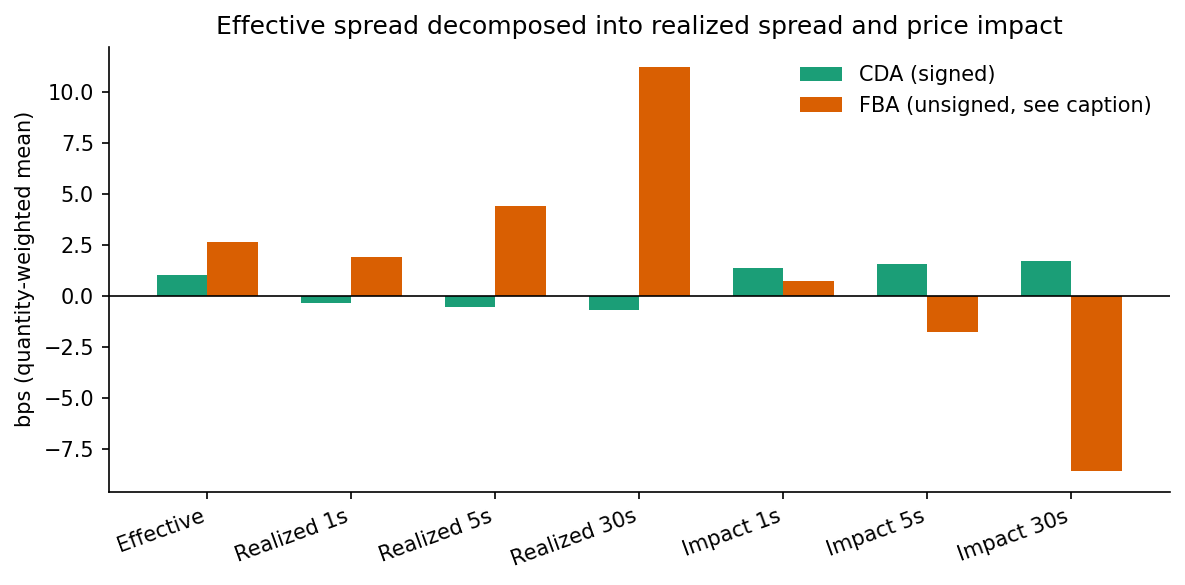
\includegraphics[width=0.95\textwidth]{figures/fig_spreaddecomp.png}
\caption[Spread decomposition]{Effective spread decomposed into realized
spread (at three markout horizons) and price impact, mean per bucket,
CDA versus FBA over the full sample. FBA values are CDA-tick-signed, a
proxy for the missing aggressor flag.}
\label{fig:spreaddecomp}
\end{figure}

\begin{figure}[htbp]
\centering
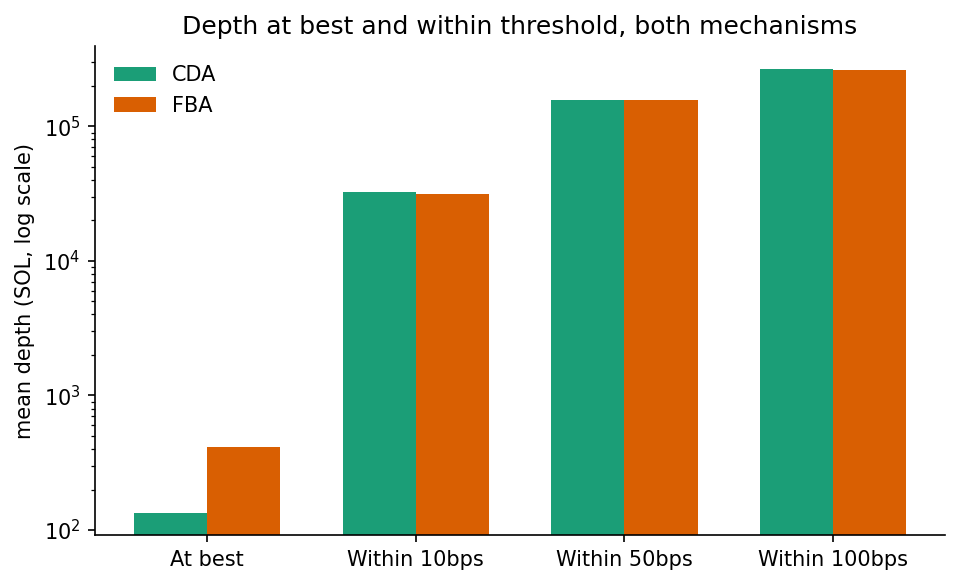
\includegraphics[width=0.7\textwidth]{figures/fig_depthcompare.png}
\caption[Depth comparison]{Mean depth at best and cumulatively within
10/50/100\,bps, CDA versus FBA (log-scale axis: depth at best is two to
three orders of magnitude smaller than the cumulative bands). The two
``at best'' figures are not directly comparable.}
\label{fig:depthcompare}
\end{figure}

\begin{figure}[htbp]
\centering
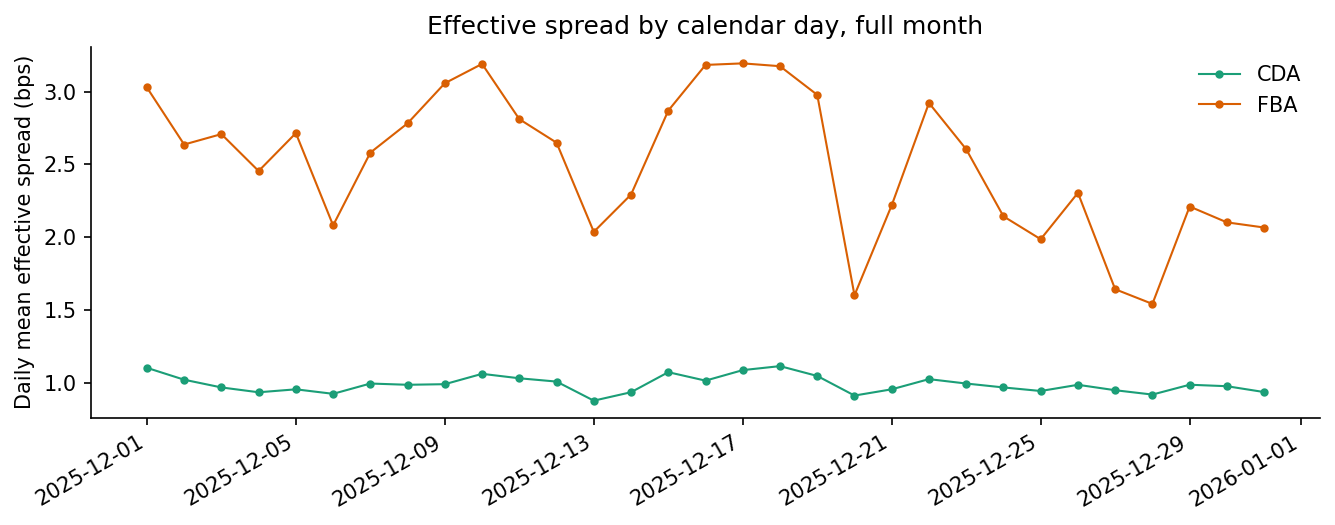
\includegraphics[width=0.95\textwidth]{figures/fig_dailytrend.png}
\caption[Daily effective spread, full month]{Daily mean effective
spread, CDA versus FBA (CDA-tick-signed), across all 31 days. The FBA's
near-zero level holds on every day, not only in the pooled mean.}
\label{fig:dailytrend}
\end{figure}

\section{RQ2.2: Price Discovery and Market Quality}
\label{sec:res22}

\Cref{tab:res22} reports the price discovery metrics.

\begin{table}[htbp]
\centering
\caption[RQ2.2 results]{Price discovery under both mechanisms. Paired
differences (FBA$-$CDA), mean (Newey--West HAC standard error in
parentheses), with $p$-values where both engines report the metric;
$n$ as in \Cref{tab:res21}. For Kyle's lambda the CDA and FBA columns are
the two slopes on the same venue flow, the difference is the slope of the
engines' difference in price change (\Cref{sec:formularq22}), and $n$ is
the number of seconds with venue flow.}
\label{tab:res22}
\small
\begin{tabularx}{\textwidth}{@{}L c c c c c@{}}
\toprule
\textbf{Metric} & \textbf{CDA} & \textbf{FBA} & \textbf{Diff.} &
\textbf{$p$} & \textbf{$n$}\\
\midrule
Intra-interval price dispersion (bps) & \ResDispersionCda & \ResDispersionFba & \ResDispersionDiff\ (\ResDispersionHacSe) & \ResDispersionP & \ResDispersionNPaired\\
Kyle's lambda, same second (bps per 1{,}000 SOL) & \ResCommonFlowLambdaCda & \ResCommonFlowLambdaFba & \ResCommonFlowLambdaDiff\ (\ResCommonFlowLambdaHacSe) & \ResCommonFlowLambdaP & \ResCommonFlowLambdaNPaired\\
Kyle's lambda, 5\,s (bps per 1{,}000 SOL) & \ResCommonFlowLambdaFiveSCda & \ResCommonFlowLambdaFiveSFba & \ResCommonFlowLambdaFiveSDiff\ (\ResCommonFlowLambdaFiveSHacSe) & \ResCommonFlowLambdaFiveSP & \ResCommonFlowLambdaFiveSNPaired\\
Matched-timestamp volatility, daily RMS (bps) & \ResMatchedVolCda & \ResMatchedVolFba & \ResMatchedVolDiff\ (\ResMatchedVolHacSe) & \ResMatchedVolP & \ResMatchedVolNPaired\\
\bottomrule
\end{tabularx}
\end{table}

\textbf{Volatility.} Volatility within a bucket cannot be compared, because
the FBA trades at most once per bucket ($n=\ResRealizedVolNPaired$ of
2{,}678{,}400 buckets). Matched-timestamp volatility replaces it. Both
engines traded in \ResMatchedVolIntersectionN\ buckets
(\ResMatchedVolIntersectionPct\%), about four times the
\ResMatchedVolIndependenceBaselinePct\% that two unrelated series with
trades in roughly 23\% of buckets would share by chance, so both engines
react to the same bursts of orders. Price changes between consecutive
matched buckets (\ResMatchedVolReturnsN\ changes) cover exactly the same
instants for both engines, and their daily root mean square is similar for
both, slightly higher for the FBA (\ResMatchedVolFba\ against
\ResMatchedVolCda\,bps, $p$ \ResMatchedVolP\ over $n=\ResMatchedVolNPaired$
days, \ResMatchedVolWindowsExcluded\ days excluded; \Cref{fig:matchedvol}).
The prediction that batching dampens price moves (\Cref{tab:theorylinks})
is therefore not borne out at $\tau = 1$\,s.
The measure covers the busier seconds in which both engines trade; it is a
comparison on common ground, not a volatility estimate for the whole month.

\begin{figure}[htbp]
\centering
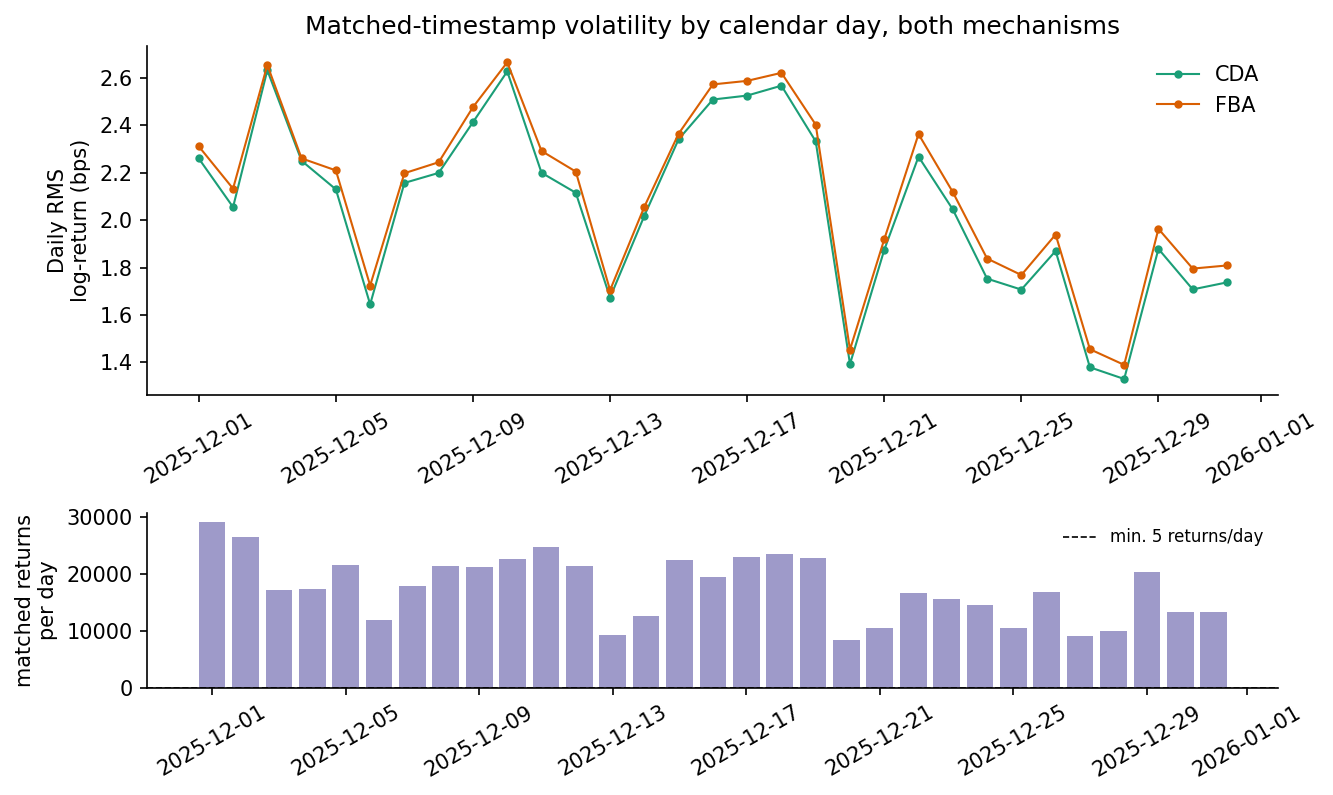
\includegraphics[width=0.95\textwidth]{figures/fig_matchedvol.png}
\caption[Matched-timestamp volatility by day]{Matched-timestamp
volatility by calendar day (top), and the number of matched returns each
day was built from against the 5-return exclusion floor (bottom).}
\label{fig:matchedvol}
\end{figure}

\textbf{Intra-interval price dispersion} is the spread of trade prices
within one second. It is \ResDispersionCda\,bps for the CDA and practically
zero for the FBA, as uniform pricing implies: exactly zero in
\DispersionFbaExactZeroPct\% of the intervals in which both engines traded,
the rest being seconds that received trades from two batch clears
(\Cref{sec:testresets}).

\textbf{Kyle's lambda.} Both engines' prices follow the venue's net taker
flow (\Cref{fig:kylelambda}, left): net buying raises the price and net
selling lowers it, as adverse selection predicts. Measured 5\,s after the
flow, the two engines respond by the same amount,
\ResCommonFlowLambdaFiveSCda\ against \ResCommonFlowLambdaFiveSFba\,bps per
1{,}000 SOL ($p$ \ResCommonFlowLambdaFiveSP). Within the same second, the
FBA's price moves more (\ResCommonFlowLambdaFba\ against
\ResCommonFlowLambdaCda, $p$ \ResCommonFlowLambdaP). The figure shows
that this gap comes only from the seconds with the very largest flows; in
every other range of flow the two curves lie on top of each other. Part
of it is also a matter of measurement: within one second the CDA's price
is a VWAP, an average along the path its trades took, while the FBA
trades once, at the price the batch ends on. The 5\,s value, read once
both prices have settled, is therefore the cleaner comparison. Batching
neither hides order flow from the price nor makes the price overreact to
it. Theory predicts that the FBA's price should react \emph{less} to
one-sided flow (\Cref{tab:theorylinks}); the replay does not show this. The CDA's own per-sweep estimate, \ResKyleLambdaCda\,bps per SOL of a
sweep's executed quantity, describes the CDA alone
(\Cref{sec:formularq22}).

\begin{figure}[htbp]
\centering
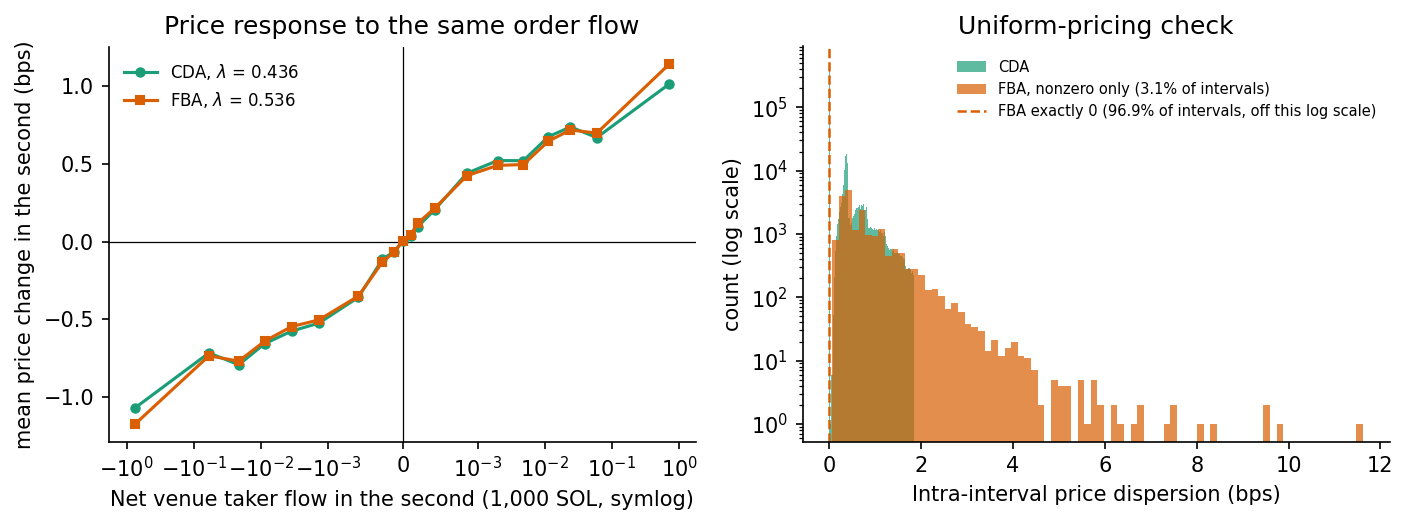
\includegraphics[width=0.95\textwidth]{figures/fig_kylelambda.png}
\caption[Kyle's lambda and the uniform-pricing check]{Left: mean price
change of each engine within the second, against the venue's net taker
flow in that second, in 20 bins of equal count (horizontal axis
symmetric-logarithmic); the legend gives the pooled same-second slopes.
Right: distribution of
intra-interval price dispersion (log-scale count axis, since the FBA's
near-total mass at exactly zero would otherwise flatten everything else);
CDA's full distribution against only the small nonzero minority of FBA
intervals. Shares in the legend are over every interval in which the FBA
traded, so they differ slightly from the share in the text, which counts
only intervals where both engines traded.}
\label{fig:kylelambda}
\end{figure}

\begin{figure}[htbp]
\centering
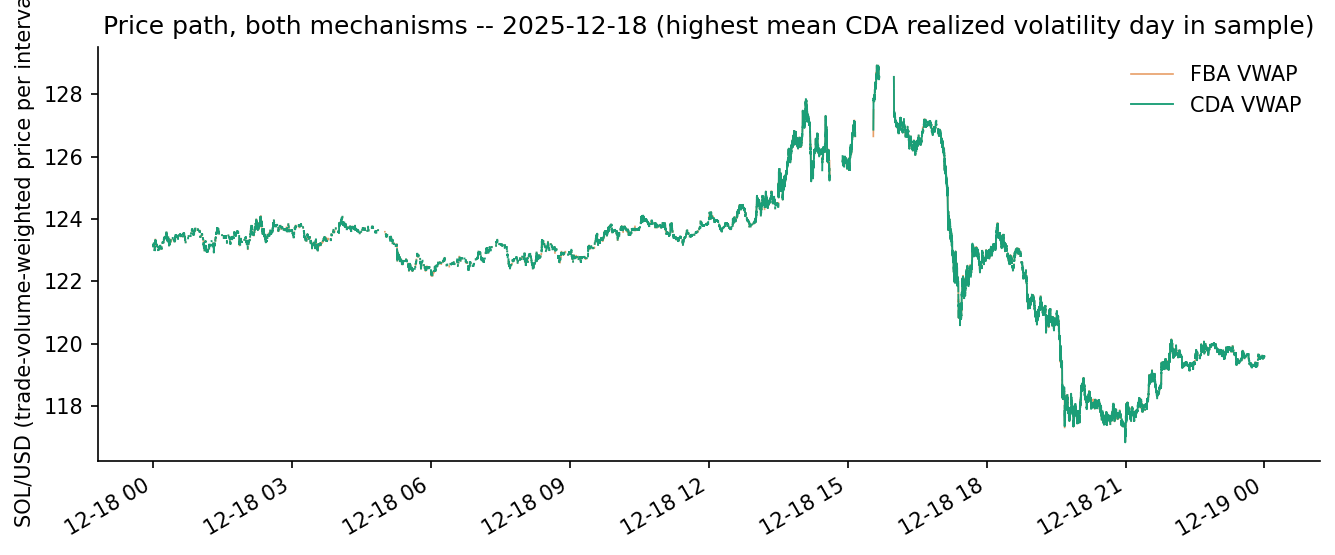
\includegraphics[width=0.95\textwidth]{figures/fig_pricepaths.png}
\caption[Price paths, both mechanisms]{CDA and FBA price paths, as the
VWAP of each one-second interval, the price series the two engines have in
common, over \PricepathsDay. This is the day with the highest mean CDA
realized volatility among the days on which at least 80\% of the
one-second buckets have a value, so that a day with little data cannot be
selected by one extreme observation. No external reference price is
available at one-second resolution to plot alongside; at an hourly scale
both prices track the spot price closely (\Cref{sec:testprice}).}
\label{fig:pricepaths}
\end{figure}

\textbf{Price paths.} The two engines' prices track each other closely
(\Cref{fig:pricepaths,fig:pricediff}). Over \PriceDiffN\ intervals in which
both traded, the FBA-minus-CDA VWAP difference has a median of
\PriceDiffMedianBps\,bps, a mean of \PriceDiffMeanBps\,bps and a standard
deviation of \PriceDiffStdBps\,bps. The gap widens only in fast markets: its
size correlates \PriceDiffVolCorr\ with CDA realized volatility, against
under 0.25 with either engine's trade count. The reason is mechanical. The
CDA's VWAP averages every fill as the book is swept within the second,
while the FBA clears once at one price, so in a fast market the two
definitions of ``the price of this second'' can differ by tens of bps
without either being wrong.

\begin{figure}[htbp]
\centering
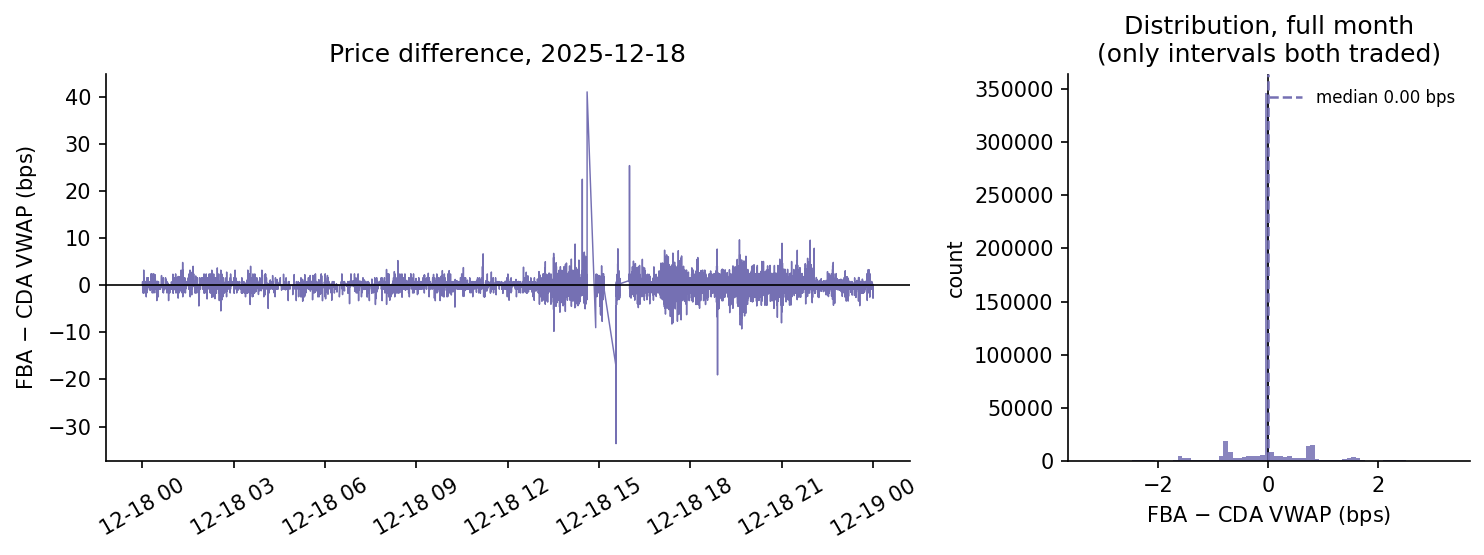
\includegraphics[width=0.95\textwidth]{figures/fig_pricediff.png}
\caption[Price difference, FBA minus CDA]{Left: the FBA-minus-CDA VWAP
difference in bps, same day as \Cref{fig:pricepaths}. Right: its
distribution pooled over every interval in the month where both engines
traded, clipped at the 0.5th/99.5th percentiles for legibility.}
\label{fig:pricediff}
\end{figure}

\section{RQ2.3: Execution}
\label{sec:res23}

\Cref{tab:res23} reports the execution metrics.

\begin{table}[htbp]
\centering
\caption[RQ2.3 results]{Execution under both mechanisms, plus engine controls. Diff.\ is mean
(Newey--West HAC standard error in parentheses); $n$ as in
\Cref{tab:res21}.}
\label{tab:res23}
\small
\begin{tabularx}{\textwidth}{@{}L c c c c c@{}}
\toprule
\textbf{Metric} & \textbf{CDA} & \textbf{FBA} & \textbf{Diff.} & \textbf{$p$} & \textbf{$n$}\\
\midrule
Executed volume (SOL, per interval, mean) & \ResExecVolumeCda & \ResExecVolumeFba & \ResExecVolumeDiff\ (\ResExecVolumeHacSe) & \ResExecVolumeP & \ResExecVolumeNPaired\\
Trade count (per interval, mean) & \ResTradeCountCda & \ResTradeCountFba & \ResTradeCountDiff\ (\ResTradeCountHacSe) & \ResTradeCountP & \ResTradeCountNPaired\\
Avg.\ time to execution (s) & \ResTimeToExecCda & \ResTimeToExecFba & \ResTimeToExecDiff\ (\ResTimeToExecHacSe) & \ResTimeToExecP & \ResTimeToExecNPaired\\
Trader surplus (USD, per interval) & \ResTraderSurplusCda & \ResTraderSurplusFba & \ResTraderSurplusDiff\ (\ResTraderSurplusHacSe) & \ResTraderSurplusP & \ResTraderSurplusNPaired\\
\midrule
\multicolumn{6}{@{}l}{\emph{Engine controls}}\\
Throughput (messages/s) & \ResThroughputCda & \ResThroughputFba & \ResThroughputDiff\ (\ResThroughputHacSe) & \ResThroughputP & \ResThroughputNPaired\\
Mean clearing/match latency ($\mu$s) & \ResClearingLatencyCda & \ResClearingLatencyFba & \ResClearingLatencyDiff\ (\ResClearingLatencyHacSe) & \ResClearingLatencyP & \ResClearingLatencyNPaired\\
\bottomrule
\end{tabularx}
\end{table}

\textbf{Executed volume} is not statistically different (\ResExecVolumeCda\
against \ResExecVolumeFba\,SOL per interval, $p$ \ResExecVolumeP); over the
month this is \$\SampleCdaNotional\ against \$\SampleFbaNotional\ of
notional (\Cref{tab:sample}). Both engines can only trade the orders that
were submitted, so this row checks the replay more than it describes the
mechanism.

\textbf{Trade count} is slightly higher for the FBA (\ResTradeCountFba\
against \ResTradeCountCda\ trades per interval, $p$ \ResTradeCountP). With
the same volume this means slightly smaller trades, consistent with one
clearing price splitting a large order among several counterparties.

\textbf{Time to execution} is the clearest cost of batching:
\ResTimeToExecFba\,s for the FBA against \ResTimeToExecCda\,s for the CDA, a
gap of \ResTimeToExecDiff\,s ($p$ \ResTimeToExecP). Waiting for the next
clear explains at most one second of it; the rest comes from orders that
stay unmatched for longer, because most batches do not cross:
\FbaEmptyBatchShare\% of all one-second batches clear no trade at all,
because no buy limit in them reaches any sell limit.

\textbf{Trader surplus} is marginally higher for the FBA
(\ResTraderSurplusFba\ against \ResTraderSurplusCda\,USD per interval, $p$
\ResTraderSurplusP). The difference does not come from uniform pricing as
such: on a trade between two limit orders, the buyer's and the seller's
improvement add up to the gap between their limits whatever the trade price
(\Cref{sec:priceimprovement}). It comes from a slightly different set of
matched orders, and from trades with a market order, whose side has no
limit and contributes nothing, so that only the limit side's improvement,
which does depend on the price, is counted (\Cref{sec:metrics23}).

\textbf{Engine controls} show whether each engine would keep up with the
order flow in real time; they do not bear on any other result
(\Cref{sec:limitsreplay}). The mean latency (\ResClearingLatencyCda\,$\mu$s
for the CDA against \ResClearingLatencyFba\,$\mu$s for the FBA) times one
order against one whole batch, which also re-evaluates every rolled-over
order, so its three-orders-of-magnitude gap reflects what is timed.
Throughput, which divides the same message count by computing time, is the
fairer comparison: \ResThroughputCda\ against \ResThroughputFba\ messages
per second of computing time, under four times apart. Both engines stay far
inside real-time needs: an FBA clear of about 2\,ms is three orders of
magnitude shorter than the one-second interval it has to fit into
(\Cref{fig:latencycontrol}).

\begin{figure}[htbp]
\centering
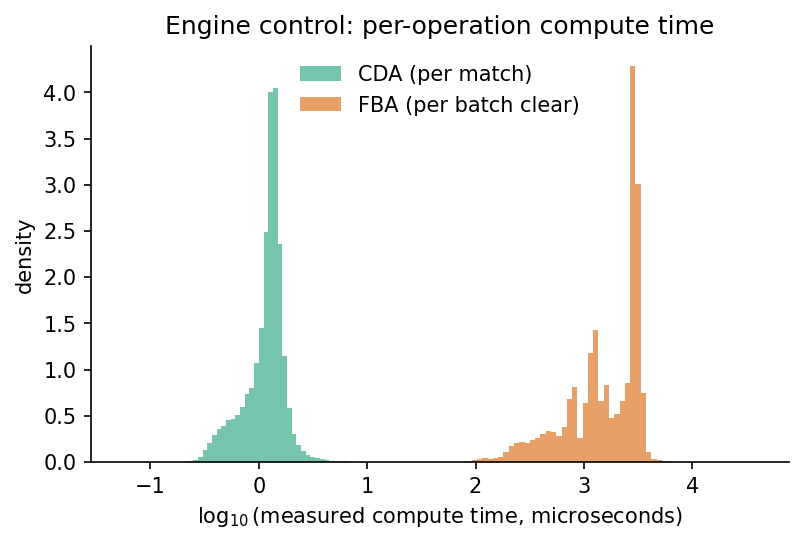
\includegraphics[width=0.95\textwidth]{figures/fig_latencycontrol.png}
\caption[Engine-control: compute latency]{Distribution of measured
compute time per operation, CDA (per message) versus FBA (per batch
clear); log scale. A control, not a market-quality result.}
\label{fig:latencycontrol}
\end{figure}

\section{Conclusions from the Simulation}
\label{sec:res_summary}

\paragraph{Main conclusion.} When the same month of SOL order flow is
cleared in one-second batches instead of continuously, \emph{how much}
trades and \emph{at what price} stay the same, but \emph{who bears the cost
of trading} changes. In the continuous market, resting orders pay a
systematic adverse-selection cost to better-informed orders; in the batch
market, no such one-sided cost is found. The batch market pays for this
with slightly less depth, longer execution times and batches that mostly
do not cross.

\Cref{tab:rq2answers} gives the answer to each part of RQ2 together with the
evidence behind it.

\begin{table}[htbp]
\centering
\caption[Answers to RQ2]{Answers to the three parts of RQ2, with the key
evidence (CDA value against FBA value).}
\label{tab:rq2answers}
\small
\begin{tabularx}{\textwidth}{@{}p{2.6cm} L p{5.4cm}@{}}
\toprule
\textbf{Question} & \textbf{Answer} & \textbf{Key evidence (CDA vs.\ FBA)}\\
\midrule
RQ2.1 Liquidity and transaction costs &
The one-sided cost that resting orders pay in the CDA does not appear in
the FBA. Standing liquidity is slightly lower in the FBA, not higher. &
effective spread \ResEffectiveSpreadCda\ vs.\ \ResEffectiveSpreadFba\,bps;
price impact at 30\,s \ResPriceImpactThirtySCda\ vs.\ \ResPriceImpactThirtySFba\,bps;
depth within 10\,bps \ResDepthWithinTenBpsCda\ vs.\ \ResDepthWithinTenBpsFba\,SOL;
Amihud \ResAmihudCda\ vs.\ \ResAmihudFba\\
\addlinespace
RQ2.2 Price discovery and market quality &
Both engines discover the same price and respond equally to the same
order flow; uniform pricing removes price dispersion within a second, and
volatility is slightly higher in the FBA. &
VWAP difference: median \PriceDiffMedianBps\,bps;
Kyle's lambda at 5\,s \ResCommonFlowLambdaFiveSCda\ vs.\ \ResCommonFlowLambdaFiveSFba\,bps per 1{,}000 SOL;
dispersion \ResDispersionCda\ vs.\ \ResDispersionFba\,bps;
daily volatility \ResMatchedVolCda\ vs.\ \ResMatchedVolFba\,bps\\
\addlinespace
RQ2.3 Execution &
The same volume trades, but orders wait longer, and most one-second
batches do not cross. &
volume \ResExecVolumeCda\ vs.\ \ResExecVolumeFba\,SOL/s ($p=\ResExecVolumeP$);
time to execution \ResTimeToExecCda\ vs.\ \ResTimeToExecFba\,s;
\FbaEmptyBatchShare\% of FBA batches empty\\
\bottomrule
\end{tabularx}
\end{table}

From these answers the simulation supports three conclusions.

\begin{enumerate}
  \item \textbf{Batching moves the cost of trading, not the volume or the
  price.} In the CDA the realized spread is negative and the price impact
  grows from \ResPriceImpactOneSCda\ to \ResPriceImpactThirtySCda\,bps
  between 1 and 30\,s: a resting order loses on average once the price has
  absorbed what the trade revealed. Kyle's lambda shows that the same net
  order flow moves both engines' prices by the same amount within 5\,s
  (\ResCommonFlowLambdaFiveSCda\ against \ResCommonFlowLambdaFiveSFba\,bps
  per 1{,}000 SOL), so the information reaches the price in both
  mechanisms; what differs is who pays for it. In the FBA all three spread
  measures stay near zero on every
  day of the month, while volume and price match the CDA. Uniform clearing
  is the mechanism that predicts a lower cost: every order in a batch trades
  at one price set after all orders are in, so there is no stale quote to
  pick off. That the cost falls to about zero, rather than merely lower, is
  more than theory predicts and rests on the estimated trade direction
  (\Cref{sec:limitssign}).
  \item \textbf{At one second, the batch market is too thin to work as
  intended.} \FbaEmptyBatchShare\% of batches clear no trade, which is why
  execution takes \ResTimeToExecDiff\,s longer on average. The FBA is also
  slightly thinner, not deeper, even though its depth is read just before
  the close, when it is overstated (\Cref{sec:limitscomparable}). The
  pooling of liquidity that batching promises needs more two-sided flow per
  batch than one second of this market provides.
  \item \textbf{Several results confirm the rule rather than add new
  findings.} Price dispersion within a second disappears, trader surplus
  barely changes (\ResTraderSurplusCda\ against \ResTraderSurplusFba\,USD
  per second), as the transfer argument of \Cref{sec:priceimprovement}
  implies. These results show that the replay behaves as specified.
\end{enumerate}

\paragraph{What the simulation does not conclude.} It does not show that
batching removes adverse selection: the FBA's trade direction is estimated,
so the result is that no one-sided cost is found, not that the cost is zero
(\Cref{sec:limitssign}). It does not show how participants would behave
under batching, because the replayed orders were never submitted to a batch
market (\Cref{sec:limitsbehaviour}). And it does not show whether a longer
interval would fill the batches without losing the first conclusion, because
only $\tau = 1$\,s was run.

\section{Limits of the Comparison}
\label{sec:metricreliability}

This section is the one place where the limits on reading the results are
set out. They come from four sources: an estimated trade direction,
metrics that cannot be compared across engines or are compared only with a
caveat, behaviour the replay cannot show, and the fidelity of the replay
itself. \Cref{tab:confidence} closes with how
far each metric family can be relied on.

\subsection{The FBA's Trade Direction Is Estimated}
\label{sec:limitssign}

Effective spread, realized spread and price impact need to know which side
of a trade initiated it. The CDA records this; in the FBA no order crosses
another's quote, so the direction is estimated with a tick rule applied to
the CDA's price series (\Cref{sec:metrics21}). Signing the FBA with its own
prices would be circular. This construction limits the FBA values in four
ways.

\begin{itemize}
  \item \textbf{The rule is imprecise.} Even on its home ground, with
  trade-level data from a single market, the tick rule classifies only
  about 78\% of trades correctly \citep{ellis2000accuracy}. Borrowing the
  sign from the \emph{other} engine's prices adds further error.
  \item \textbf{A near-zero average has two readings.} The raw FBA deviation
  has no sign, and multiplying it by an estimated sign gives an average near
  zero whenever that sign is nearly unrelated to the true direction. Either
  the FBA's trades carry no systematic direction, so there is no cost to
  find, or the CDA's tick is a poor guide to the direction of an FBA batch,
  so the estimate cannot find a cost that is there. Without an aggressor
  flag for the FBA the data cannot separate the two.
  \item \textbf{The three measures are one result.} All three FBA values
  apply the same sign to the same trades, so their agreement is not three
  independent confirmations; a bias in the sign would move all three
  together.
  \item \textbf{The result is stronger than theory predicts.} Theory
  predicts a \emph{reduction} in price impact, not its disappearance
  (\Cref{sec:spread-decomposition}), which is a further reason to read the
  near-zero values only as far as the estimate allows.
\end{itemize}

What survives is the CDA side, which needs no estimate, and the weaker
statement that under the best available direction the FBA shows no
one-sided cost of the kind the CDA shows.

\subsection{Which Metrics Can Be Compared}
\label{sec:limitscomparable}

Most metrics are defined the same way for both engines and are compared
directly: executed volume, trade count and VWAP, depth within a
threshold, Amihud illiquidity, intra-interval dispersion,
matched-timestamp volatility, Kyle's lambda, time to execution and trader
surplus. The spread decomposition is compared too, with the limits set out
in \Cref{sec:limitssign}. Two metrics cannot be compared at all, and three
are compared with a caveat.

\paragraph{Not comparable.} \textbf{Depth at best} compares one CDA price
level with the whole eligible side of the FBA schedule at the clearing
price, $(D(\clr) + S(\clr))/2$, which adds up all orders priced at or
better than $\clr$. The FBA's higher value is a consequence of this
definition, not of more liquidity, so the two are reported but not
compared. \textbf{Realized volatility within a bucket} needs two prices in
one second, which the FBA almost never has; matched-timestamp volatility
replaces it.

\paragraph{Compared with a caveat.} \textbf{Depth within a threshold}
carries the depth result. Its one asymmetry, that the FBA's value is read
just before the batch clears and so includes orders about to execute, can
only make the FBA look deeper, so the finding that it is thinner holds
with margin. \textbf{Quoted spread} is computed correctly for both
engines, but the FBA's is read from the leftover orders just after a
clear, which is not the same kind of object as a CDA book that has
continuously matched everything it could (\Cref{sec:fbavscda,app:comparability}).
It is therefore weaker evidence about liquidity than depth within a
threshold. \textbf{Kyle's lambda} regresses both engines on the same
regressor, the venue's own net taker flow per second
(\Cref{sec:formularq22}), so the two slopes are directly comparable. Two
limits remain. The regressor is the flow that executed on the venue, not
on either simulated engine: the CDA replays the same orders and its volume
follows the venue's over time, though at about twice its level
(\Cref{sec:testfidelity}), while in the FBA the same orders may trade in a
different second or not at all. And within one second the CDA's price is a
VWAP and the FBA's a single clearing price, which can widen the
same-second gap; the 5\,s horizon avoids this.

\subsection{Behaviour the Replay Cannot Show}
\label{sec:limitsbehaviour}

The replayed orders were submitted to Hyperliquid's continuous engine, not
in reaction to batching (\Cref{sec:testable}). Every result is therefore
the mechanical effect of the batch rule on fixed historical orders.
Timing orders against a real, predictable batch close
(\Cref{sec:priceimprovement}), requoting by market makers, bid shading
under price uncertainty and size inflation under a rule that rewards it
all need participants who can respond to the mechanism, so none of them
can be measured here.

\subsection{Fidelity of the Replay}
\label{sec:limitsreplay}

\begin{itemize}
  \item \textbf{Volume level.} The replay does not enforce post-only orders
  or self-trade prevention, so it trades about twice the venue's recorded
  volume (\Cref{sec:testfidelity}). Both engines receive this same input, so
  it does not favour either side of a paired comparison, but absolute
  volume, trade-count and latency levels describe the replay, not the live
  market.
  \item \textbf{Rounding.} Sizes are rounded to whole SOL, and orders below
  0.5\,SOL are skipped for both engines (\Cref{sec:dataset}).
 
  \item \textbf{Implementation.} A difference could in principle come from
  how well each engine is implemented. This is checked by the shared order
  representation and metrics code, the independent reference implementation
  and the test suites (\Cref{app:testing}); convergence of the FBA to the
  CDA as $\tau \to 0$, the strongest such check, was not run.
  \item \textbf{Engine controls.} The replay runs on the data's timestamps,
  so computing speed cannot change any market metric. Throughput and
  latency are wall-clock measurements and the only two of the 35 output
  columns that are not reproduced bit for bit across runs
  (\Cref{sec:testdeterminism}).
\end{itemize}

\begin{table}[htbp]
\centering
\caption[How far each metric can be relied on]{How far each metric family
can be relied on, and why.}
\label{tab:confidence}
\small
\begin{tabularx}{\textwidth}{@{}p{4.2cm} p{2.4cm} L@{}}
\toprule
\textbf{Metric family} & \textbf{Reliance} & \textbf{Reason}\\
\midrule
Executed volume, trade count, VWAP & high & read directly off executed trades, same definition for both engines\\
Time to execution, trader surplus & high & same definition for both engines, computed from each engine's own fills\\
Depth within a threshold, Amihud & high & same definition for both engines; the one asymmetry favours the FBA\\
Intra-interval dispersion, matched-timestamp volatility & high & same definition, and the volatility uses the same instants for both engines\\
Kyle's lambda, 5\,s & high & same regressor (venue flow) and same definition for both engines\\
Kyle's lambda, same second & moderate & CDA price is a VWAP within the second, the FBA's a single clearing price\\
Spread decomposition, CDA side & high & observed trade direction\\
Spread decomposition, FBA side & low & estimated direction; shows only that no one-sided cost is found\\
Quoted spread & moderate & FBA value read from leftover orders, not a book\\
Depth at best & not comparable & different objects in the two engines\\
Realized volatility within a bucket & not comparable & the FBA has at most one price per second; replaced by matched-timestamp volatility\\
Throughput, latency & feasibility only & no effect on market metrics in an event-time replay\\
\bottomrule
\end{tabularx}
\end{table}
